\section{Data Transfer}

The system relies of on wireless data transfer to send traffic data recorded by a node back to the central database. It is also useful to be able to transmit a live video feed from each node to the graphical interface so that a user may observe what the node sees in real time Presently data transfer occurs only on a local area network and so nodes and the central machine housing the database must be on the same network. Making the network wireless was an important consideration as it allows for more flexible and lightweight node installation.

\subsection{Video Feed}

The video feed is shared with the user interface via a simple Flask \cite{flask} application that's only functionality is uploading new images to a URL on the local network, the URL is simply embedded in the user interface as an image. Flask is a lightweight web framework for custom web services which made it optimal for the specific and small task of streaming images from a Raspberry Pi on a local network.


\subsection{Traffic Statistics}

Traffic statistics are sent to the database every 30 seconds. A simple custom library was written to interface with the database informed by the "MySQLTutorial" series \cite{mysqltutorial} that utilizes the MySQLConnector class \cite{mysqlconnector}. The connection using this library is by default set to transfer control protocol (TCP) which is well suited to sending small packets of data. 

\begin{figure}[H]
    \centering
    \centering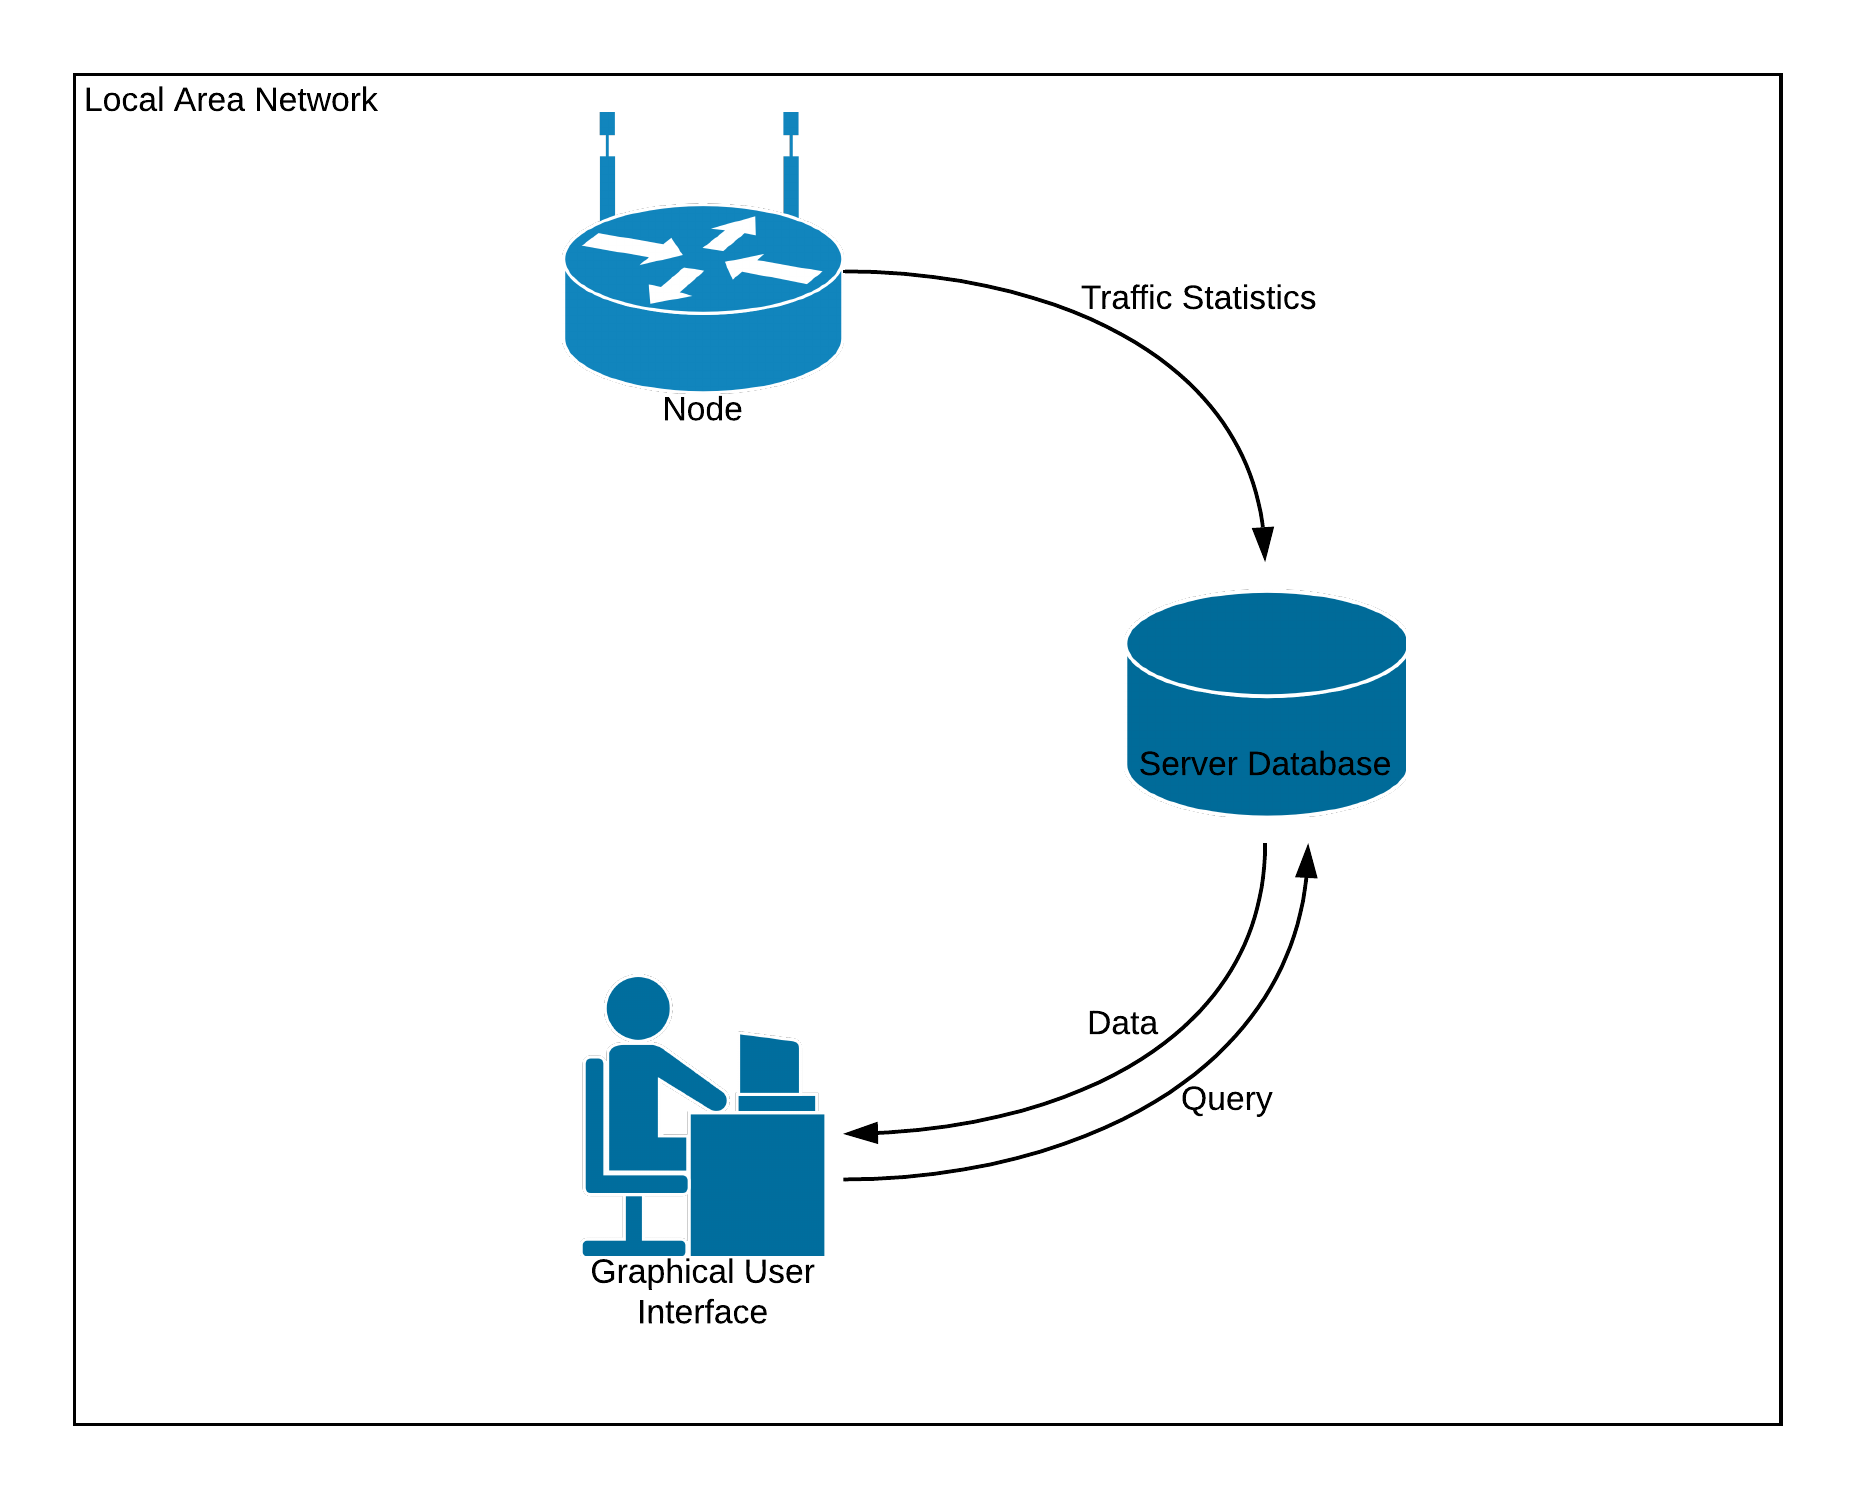
\includegraphics[width = 0.8\textwidth]{design/networking/network_diagram}
    \caption{High level operation of system network.}
    \label{fig:network_diagram}
\end{figure}